% Metódy inžinierskej práce
\documentclass[10pt,twoside,slovak,a4paper]{article}										%%%%%%%%%%%%%%%
																		%				         %
\usepackage[slovak]{babel}														%   Oliver Ondruš 6.11.2021     %
%\usepackage[T1]{fontenc}														%    	         ID:116261	         %
\usepackage[IL2]{fontenc} 														%                                                %
\usepackage[utf8]{inputenc}														%%%%%%%%%%%%%%%
\usepackage{url} 
\usepackage{hyperref} 
\usepackage{graphicx}
\usepackage{cite}
%\usepackage{times}
\pagestyle{headings}

\title{Športové tréningy a ich modelovanie vo virtuálnej realite\thanks{Semestrálny projekt v predmete Metódy inžinierskej práce, ak. rok 2020/21, vedenie: Ing. MLYNAROVIČ Vladimír  PhD.}} 
\author{Oliver Ondruš\\[2pt]
	{\small Slovenská technická univerzita v Bratislave}\\
	{\small Fakulta informatiky a informačných technológií}\\
	{\small \texttt{xondruso@stuba.sk}}
	}

\date{\small 6.11.2021} 
\begin{document}
\maketitle

\begin{abstract}
V článku sa chcem zaoberať objasnením funkčnosti a metodológie reakčných a motorických tréningových programov vo virtuálnej realite (ďaľej už len VR) v 3D simulovanom priestore , ktoré majú napomáhať vrcholovým alebo amatérskym športovcom v rozvoji svojich fyzických , mentálnych a kognitývnych schopností ako sú napríklad rozpoznávanie objektov , zlepšenie reakcií na fyzické podnety , konanie správnych rozhodnutí v správny čas a ich následné porovnanie s výsledkami v reálnom svete. Spresnie architektúry daných systémov od zostavenia programu po skonštruovanie do použiteľnej formy v priestore. Uvediem výsledky z výskumov na dobrovoľníkoch z profesionálnej a amatérskej sféry , dopad na terajší športový systém trénovania profesionálnych a neprofesionálnych atlétov v rôznych odvetviach športu.
\end{abstract}
\textbf{Klúčové slová :}
Virtuálna realita, šport, alternatívne tréningy, VR, šport vo virtuálnej realite, špeciálne tréningy, model virtuálnej reality, využitie virtuálnej reality

\section{Úvod}
Zlepšenie herného výkonu jednotlivca môže byť pre neho samého veľmi náročné, hlavne keď sa jedná o kolektívne športy. Človek nemá vždy prístup k veľkému ihrisku alebo dostatok spoluhráčov pre tréning, aký by potreboval. V individuálnom rozvoji mu bránia rôzne biomechanické, psychologické a fyziologické faktory. Je preto nutné lepšie porozumieť systému akcie a reakcie atlétov v ich športoch. To vyžaduje izolovanie faktorov, ktoré tvoria úlohy pre jeho hernú činnosť na danej pozícií v hre. Prehrávanie videozáznamov kvôli svojim obmedzeniam nedokáže poskytnúť dostatočne hlbokú analýzu činnosti jednotlivca v hre. Interaktívna a pohlcujúca VR môže tieto obmedzenia prekonať a pomôcť tak lepšie pochopiť športový výkon z behaviorálnej perspektívy. V nasledujúcich kapitolách si predstavíme pojem VR ,tréningy športovcov a ich adaptáciu na VR, metodológiu, modelovanie VR, potrebný hardware a pomôcky, personál, štatistiky, zhodnotenie efektivity. ~\cite{Hlavny:zdroj}
Podstatné informácie v častiach~\ref{SW} a~\ref{HW}. Pre vysvetlenie pojmu virtuálna realita sú informácie v časti~\ref{VR}. 
Záverečné zhodnotenie v časti~\ref{zaver}.
  

\section{Virtuálna realita}	\label{VR}
\subsection{História} \label{VR:hist}		
Virtuálna realita je pojem zaužívaný od roku 1987 , ktorý definoval \emph{Jaron Lanier} ~\cite{Jaron:zdroj}. Za prvý prístroj na VR sa však považuje tzv. \emph{Damaklov meč}. Bol to prístroj ktorý bol upevnený k stropu budovy kvôli svojej váhe a bol nasadený na hlavu človeka. Jeho virtuálne prostredie tvorili virtuálne miestnosti ohraničené čiarami.

\subsection {Definícia} \label{VR:now}
 Headsety pre virtuálnu realitu v dnešnej dobe dokážeme vytvoriť aj z nášho smartfónu a kartónového modelu , ktorý vieme sami zložiť. Virtuálna realita sa považuje za legitímnu vtedy, ak úplne zamestnáva všetky naše zmysly alebo primárne zmysly na vnímanie informácií (zrak, sluch). Existuje aj AR - agumentovaná či rozšírená realita. Ta predstavuje akýsi virtuálny doplnok do nášho reálneho sveta takým spôsobom ,že sme schopní vnímať svoje okolie v reálnom svete. Virtuálna realita je používaná vo veľkom v rôznych sférach .Používa sa v odvetviach produktového dizajnu, medicíny, školstva, psychológie, zábavného priemyslu, architektúry a v neposlednom rade športu.~\cite{zhrnutie:zdroj}

\subsection{Typy zariadení} \label{VR:typy}
V dnešnej dobe sa môžeme stretnúť s niekoľkými zariadeniami, ktoré su shcopné poskytovať virtuálnu realitu. Niektoré používame aj každý deň.
Typy týchto zariadenia sa môžu deliť podľa rôznych kritérii, základným delením je podla miery ponorenia jednotlivca do VR ~\cite{types:zdroj}:
\begin{itemize}
\item Nepohlcujúce zobrazovacie zariadenia
	\begin{itemize}
	\item Smartphone       
	\item Tablet
	\item Počítač
	\end{itemize}	
\item Polo-pohlcujúce zobrazovacie zariadenia
	\begin{itemize}
	\item 3D monitory
	\item Zahnuté displeje
	\item "Jaskyne"\footnote{Prázdna miestnosť v tvare kocky , v ktorej každý z povrchov , steny , podlaha a strop, možno použiť na premietanie pre ponorenie do VR}
	\end{itemize}	
\item Pohlcujúce zobrzovacie zariadenia
	\begin{itemize}
	\item "Jaskyne"
	\item Standalone zariadenia \footnote{zariadenie nevyžaduje žiadne ďaľšie externé senzory , headset a ovládanie (napr. Oculus Quest)}
	\item Statické zariadenia \footnote {zariadenie vyžaduje externé senzory pre priestor (napr.HTC VIVE)}
	\end{itemize}
\end{itemize}

\section{Software} \label{SW}
\subsection{Používané nástroje} \label{SW:tools}
Nakoľko sa VR zaoberá prevažne sférou videohier , najčastejšie používané jazyky pre programovanie softwarov pre VR sú C/C++, C\#, Java, JavaScript a Python. Často používané prostredie alebo engine pre VR je herný engine Unity3D , ktoré prevažne funguje pomocou jazykov C\# a C++. Prevažná časť týchto programov nepodporuje tzv. multiplayer nakoľko je to zatiaľ príliš komplexné na zostrojenie z dôvody náročných fyzikálnych výpočtov, ktoré by museli prebiehať aj na veľmi výkonnom zariadení 
Jedným zo základných problémov pri vytváraní simulácie vo VR je riešenie fyziky .\footnote{ prírodná veda o transformáciách energia v časopriestore a o vlastnostiach jej foriem a prejavov}.V herných enginoch je však ovládanie fyziky jednotlivých objektov jednoduchšie spracovateľné ako len holé programovanie.

\subsection{Modelovanie simulácie} \label{SW:model}
Používanie VR na analýzu športových výkonov zahŕňa 3 kroky. Prvým krokom je zaznamenanie pohybu športovca alebo športovcov v danom športe počas hry. Tieto dáta potom slúžia na animáciu NPC postáv alebo animáciu samotného športovca. Neje to však jediné vyžitie týchto dát , sú veľmi nápomocné hlavne pri porovnaní výkonov v simulovaných situáciách oproti tým v reálnom svete. V druhom kroku sa odohráva animácia samotných humanoidných NPC a užívateľa a ich následná adaptácia do nami požadovanej simulovanej situácie z reálneho sveta na ktorú sa chceme zamerať. Tretím krokom je prezentácia vo VR.

Napriek tomu že pri väčšine športov sú prvé dva kroky k vytvoreniu simulácie rovnaké pre uvedené aplikácie, tretí krok závisí od konkrétnej aplikácie , pretože každý imerzívny(pohlcujúci) zobrazovací systém má vlastné plusy a mínusy . V štúdií o hádzanej napríklad, sa musí snímaný subjekt pohybovať rovnako voľne, ako pri reálnej hre na ihrisku. Je teda použitá veľká valcová obrazovka. Keď sa napríklad pozrieme na rugby , tak sa jedná o rozoznávanie klamlivého pohybu virtuálneho modelu predstavujúceho protihráča. Preto stačí používať headsetové zariadenie teda displej namontovaný na hlave(časť~\ref{VR:typy}). ~\cite{Hlavny:zdroj}
\clearpage
\begin{figure*}[htbp]
\centering
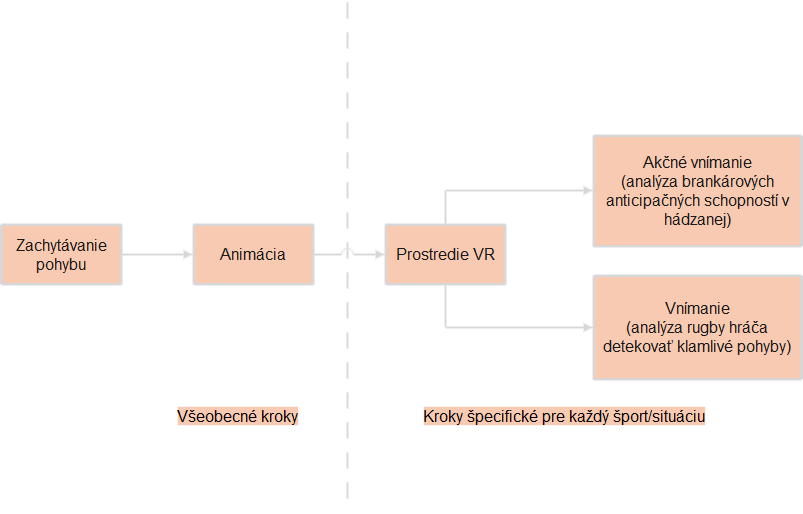
\includegraphics[scale=0.4]{model.png}
\caption{Na tomto obrázku môžeme vidieť jednoduchý projektový plán pre zostrojenie špecifickej situácie vo VR}  ~\cite{Hlavny:zdroj}
\label{fig}
\end{figure*}

\section{Hardware} \label{HW}
Hardware pre podporu VR programov sa líši v závislosti od požadovanej funkcie. Napríklad pri simulácii z hokeja je potrebné mať priestor minimálne 4x4 metre ~\cite{setuphk:zdroj}, v závislosti od toho či chceme simuláciu pre hráča alebo brankára sa prirodzene odvíja potrebné športové vybavenie ale aj vybavenie pre VR. Ak chceme simuláciu pre brankára je potrebné mať viac senzorov.2 Na ruky , v ideálnom prípade na brankárske rukavice. Dnešné programy už fungujú tak, aby dokázali rozoznať pozíciu osoby aj bez senzorov nôh (časť~\ref{SW}). A nakoniec jeden headset. Preferovaný je Oculus Quest ~\cite{headset:zdroj}(časť~\ref{VR:typy}), ale väčšina programov funguje aj na iných. Pre hráča tak isto platí 1 headset ale stačí mu len jeden senzor a to na hokejku. Oproti brankárovi teda potrebuje oveľa menej. Z športových potrieb mu takisto stačí len hokejka. Pre oboch platí že sa dá VR headset využiť aj na ľade poprípade na syntetickom ľade, kde sa dá korčuľovať. Samotné zariadenie môže fungovať aj cez herný počítač, ale konkrétne pri hokejovom programe je potrebné, ak teda využívame herný počítač, nainštalovať aj príslušné senzory do miestnosti podľa stanovených kritérií a nimi zachytávaného priestoru(časť~\ref{VR:typy}).

%Ten istý zoznam, len číslovaný:
%
%\begin{enumerate}
%\item jedna vec
%\item druhá vec
%	\begin{enumerate}
%	\item x
%	\item y
%	\end{enumerate}
%\end{enumerate}

\section{Personál} \label{PR}

\subsection{Prevádzkovateľ}\label{PR:boss}
Môj rozhovor s majiteľom firmy Sense Arena Danielom Benešom na tému Hokej vo virtuálnej realite mi odhalil veľa zaujímavosti ohľadom prevádzkovania VR služieb pre športovcov. Hlavným predajným faktorom alebo propagačným nástrojom pre tréning vo VR, je jeho veková neobmedzenosť a kompaktnosť v dnešnej podobe. V minulosti bolo jediným riešením mať k systému herný počítač alebo podobne výkonný počítač, no dnes vďaka standalone headsetom ako Oculus Quest(časť~\ref{VR:typy}) je možné používať VR trénovanie prakticky kdekoľvek , kde má človek dosť miesta.  Ďalším faktorom je, napríklad pre hokej, že človek nemusí zbierať puky, pretože fyzicky ani neexistujú a v simulácií sa po skončení "respawnujú"\footnote{znovu sa objavia} . V podobnom duchu sa nesie tak isto faktor , že vaši spoluhráči vo VR sa neunavia . Môžete preto trénovať takmer ľubovoľné cvičenia koľko vládzete. Odporúčané je však neprekračovať cca 200minut týždenne tréningov vo VR. Firma Sensa Arena si získala podporu aj v zámorí kde podpísali zmluvu so štyrmi NHL tímami a momentálne majú 1500 zákazníkov ktorý si platia mesačnú subskripciu ich produktu na doma. Prakticky je možné pre kohokoľvek si zaobstarať ich produkt aj na komerčné účely za podmienok navýšenej subskripcie.

\subsection {Užívateľ} \label{PR:user}
Užívateľ je zrejme jedinoupodmienkou , bez ktorej, sa ďalej nepohneme. Musí byť oboznámený vopred s fungovaním zariadenia a najprv podstúpiť skúšobné simulácie aby sa systém správne nastavil na jeho biometriku. Po nastavení a oboznámení môže užívateľ sám spustit simuláciu, alebo ho prevádzkovateľ upozorní na jej začiatok a typ. Pre užívateľa je častokrát možné samovoľne zastaviť simuláciu , alebo požiadať trénera aby jeho kroky skontroloval , poprípade opravil.

\subsection {Tréner} \label{PR:trendo}
Pre vrcholových športovcov je ideálne vstúpiť do tréningového procesu vo VR aj spolu so svojím trénerom. Avšak nieje to podmienkou, častokrát je samotný púrevádzkovateľ zároveň trénerom nakoľko ide vždy o špecifickú simuláciu, odborník v dnaej oblasti musí byť aj prevádzkovateľ. Preto je aj pre amatérskych športovcov možné dostať profesionálny tréning bez prítomnosti vlastného trénera.

\subsection{Adaptovatelné tréningy mimo VR} 
\begin{itemize}
\item Motorické tréningy: Hand-eye koordinacia, Celotelová koordinácia	
\item Decision-making
\item Play-tracking
\item Speed-drills: zrýchlenie, laterálna rýchlosť, výbušnosť
\item Reakčné tréningy
\item Tréningy na vylaďovanie techniky (pre brankárov v hokeji napr. box control)
\end{itemize}

\clearpage
\begin{figure*}[h]
\centering
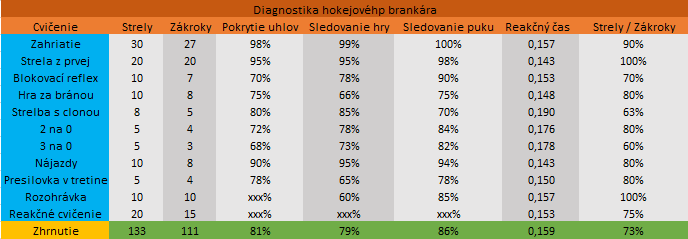
\includegraphics[scale=0.59]{tabulka.png}
\caption{Táto tabuľka znázorňuje výsledky simulácie určenej pre hokejového brankára}  ~\cite{Hlavny:zdroj}
\label{fig}
\end{figure*}

% reakcie na prednášky
\section{Reakcie na prednášky}

\paragraph{Etika a udržateľnosť. } 
Etické spôsoby a udržateľný prístup musia ovládať podľa mňa všetci, nielen inžinieri. Udržateľnosť má čestné miesto pri veľa situáciách s ktorými sa musíme, ako programátori denne stretávať. Rovnako etika musí stále byť dodržaná pri vypracovávaní zadaní, kde je plagiátorstvo prísne trestané a brané za nemorálne voči kolegom a univerzite. V neposlednom rade je dôležité aj udržiavanie mentálneho a fyzického zdravia. Ako inžinieri budeme častokrát dlhé hodiny sedieť na jednom mieste, častokrát tento spôsob pracovania môže pretrvať niekoľko rokov takže je kľúčové aby sme sa vedeli o seba starať správne. Táto prednáška nás celkom dobre oboznámila s týmito problémami.~\cite{etics:zdroj}

\paragraph{Historické súvislosti.} 
Táto prednáška bola vysoko informačného charakteru v súvislosti s históriou velikánov informatiky za posledné storočie, ktorí nás bohužiaľ opustili behom posledných dvoch rokov. Hlavne som si rozšíril obzory v tom, ako jednoduché a pre nás bežné pomôcky v každodennom živote informatika boli stvorené. To čo v dnešnej dobe považujeme za úplnú samozrejmosť a vec ktorú dokáže používať úplne každý kedysi musel niekto krvopotne vymyslieť a sfunkčniť. Ohromila ma hra Johna Conwaya „Game of life“, ktorá dokáže fungovať na minimálnych podmienkach pre hráča, čo sa týka nároku na hardware ale aj pochopenie, a popri tom dokáže vytvoriť úžasné veci, ktoré už dokážu klásť veľký tlak jak na hráča tak na hardware. Celkovo to bola veľmi zaujímavá prednáška s náhľadom do nie tak ďalekej minulosti, ktorá vyzerala úplne inak, ako tieto veci poznáme dnes. ~\cite{sedem:zdroj}

\paragraph{Spoločenské súvislosti.} 
Prednáška s dekanom fakulty bola jedna z najlepších podľa môjho usúdenia. Prejsť si všetky faktory, ktoré práca v IT zahŕňa priamo s človekom, ktorý sa v tejto sfére pohybuje dlhé roky nám určite všetkým pomohlo si trochu upratať hodnoty a myšlienky v tom, čo od nášho štúdia na FIIT očakávame. Zobral som si z prednášky veľa informácií o fungovaní v IT, ktoré mi určite budú nápomocné pri výbere môjho smerovania nielen, ako študenta, ale aj, ako pracovníka v IT sfére, ktorá ponúka nespočítateľne veľa možností uplatnenia.~\cite{naco:zdroj}


\section{Záver} \label{zaver}
Dozvedeli sme sa akým spôsobom fungujú zariadenia VR, akým štýlom sa modelujú jednotlivé situácie ktoré napomáhajú športovcom k zlepšovaniu ich fyzických , ale aj mentálnych schopností. Objasnili sme si typy zariadení a pojem VR a jej krátku hsitóriu. Bližsie sme sa pozreli na funkcie jednotlivcov z personálu okolo simulácie tréningu vo VR. Dostali sme náhľad do zákulisia firmy Sense Arena , ktorá sa zaoberá poskytovaním športových simulácií pre profesionálnych ale aj amatérskych hokejistov. Uviedli sme si nároky na hardware a software potrebný na zrealizovanie akejkoľvek simulácie za účelom zelpšiť sa v danom športe. Z pohľadu efektivity sú tieto tréningy veľmi nápomocné. Potvrdzuje to niekoľko desiatok dlhodobých štatistík a aj fakt, že sú využívané vrcholovými športovcami na regulernej báze. Bohužial kvôli rozsahu nemôžeme priblížit recenzie profesionálov a plne zhodniť efektivitu.
								%recenzie profesionalov , recenzie amaterov , moja recenzia , zhodnotenie ++ a -- , zhrnutie   
\bibliography{literatura}
\bibliographystyle{plain} 
\end{document}
